\chapter{Budowa programu}
W rozdziale trzecim zawarto informacje dotyczące budowy programu. Na początku opisana jest jego struktura w postaci diagramów. Następnie opisane są poszczególne fragmenty programu. Na końcu znajduje się opis interfejsu graficznego programu.


\section{Struktura programu}

Poniżej znajduje się opis struktury plików oraz opis zawartości poszczególnych katalogów programu.

\begin{itemize}
	\item \textbf{main.py} - zawiera w sobie główną logikę programu
	\item \textbf{staff\_detection.py} - w skład tego pliku wchodzą funkcje odpowiedzialne za detekcję pięciolinii
	\item \textbf{dewarp\_image.py} - plik zawierający całą logikę i działanie części programu odpowiedzialnej za usuwanie wypaczenia z obrazów wejściowych
	\item \textbf{image\_segmentation.py} - jest plikiem posiadającym wszystkie funkcje mające za zadanie poprawne podzielenie obrazu na mniejsze fragmenty nadające się na przekazanie dla wytrenowanego modelu uczenia maszynowego
	\item \textbf{utils.py} - przechowuje funkcje dodatkowe
	\item \textbf{setup.py} - plik konfiguracyjny 
	\item \textbf{ML\_model} - folder zawierający wytrenowany model uczenia maszynowego
\end{itemize}

\section{Diagram maszyny stanowej}

\begin{figure}
	\centering
	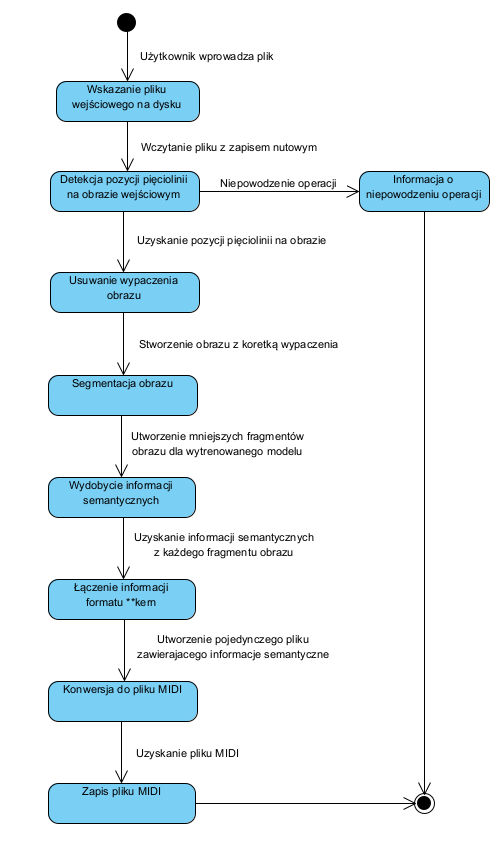
\includegraphics[width=10cm]{images/diagram-maszyny-stanowej-programu.png}
	\caption{Diagram maszyny stanowej programu.}
	\label{fig:program-state-machine}
\end{figure}


\section{Interfejs graficzny}